\subsubsection{Boot service}

The Boot service is responsible of starting the system in a graceful fashion.
It does so by dividing the start phase into two subphases, namely the
\textbf{initialization} and the \textbf{boot} phase.

Initially, this service is in a \texttt{uninitialized} state, which means the
node has received neither a marker from a neighbor node to start the
initialization phase nor it has been acknowledged by the application layer that
its initialization is finished.

If the application layer tells the middleware that it's initialized, then the
Boot service will become \texttt{initialized}. If instead an initialization
marker arrives from a neighbor, the Boot service will stay in the
\texttt{uninitialized} state, waiting for the application layer to tell it's
initialized.
If the middleware receives another marker after having received the first one,
then it will reply immediately as it had finished its initalization phase.
Finally, when the Boot service has received all the initialization markers from
its neighbors and has been acknowledged by the application layer that it is
initialized, it will enter the \texttt{booting} state (and the \textbf{boot}
phase).

In the second phase this service waits for the boot marker (a middleware-layer
message which starts the boot of the system) to arrive. When it does, the Boot
service forwards the marker to all its neighbor and wait for all of them to
reply (i.e, for them to be booted).
When all the neighbors are booted, the application layer gets booted as
well and the Boot service sends a boot marker back.

The whole process is depicted in Figure \ref{fig:mw-boot}.

\begin{figure}[H]
  \centering
  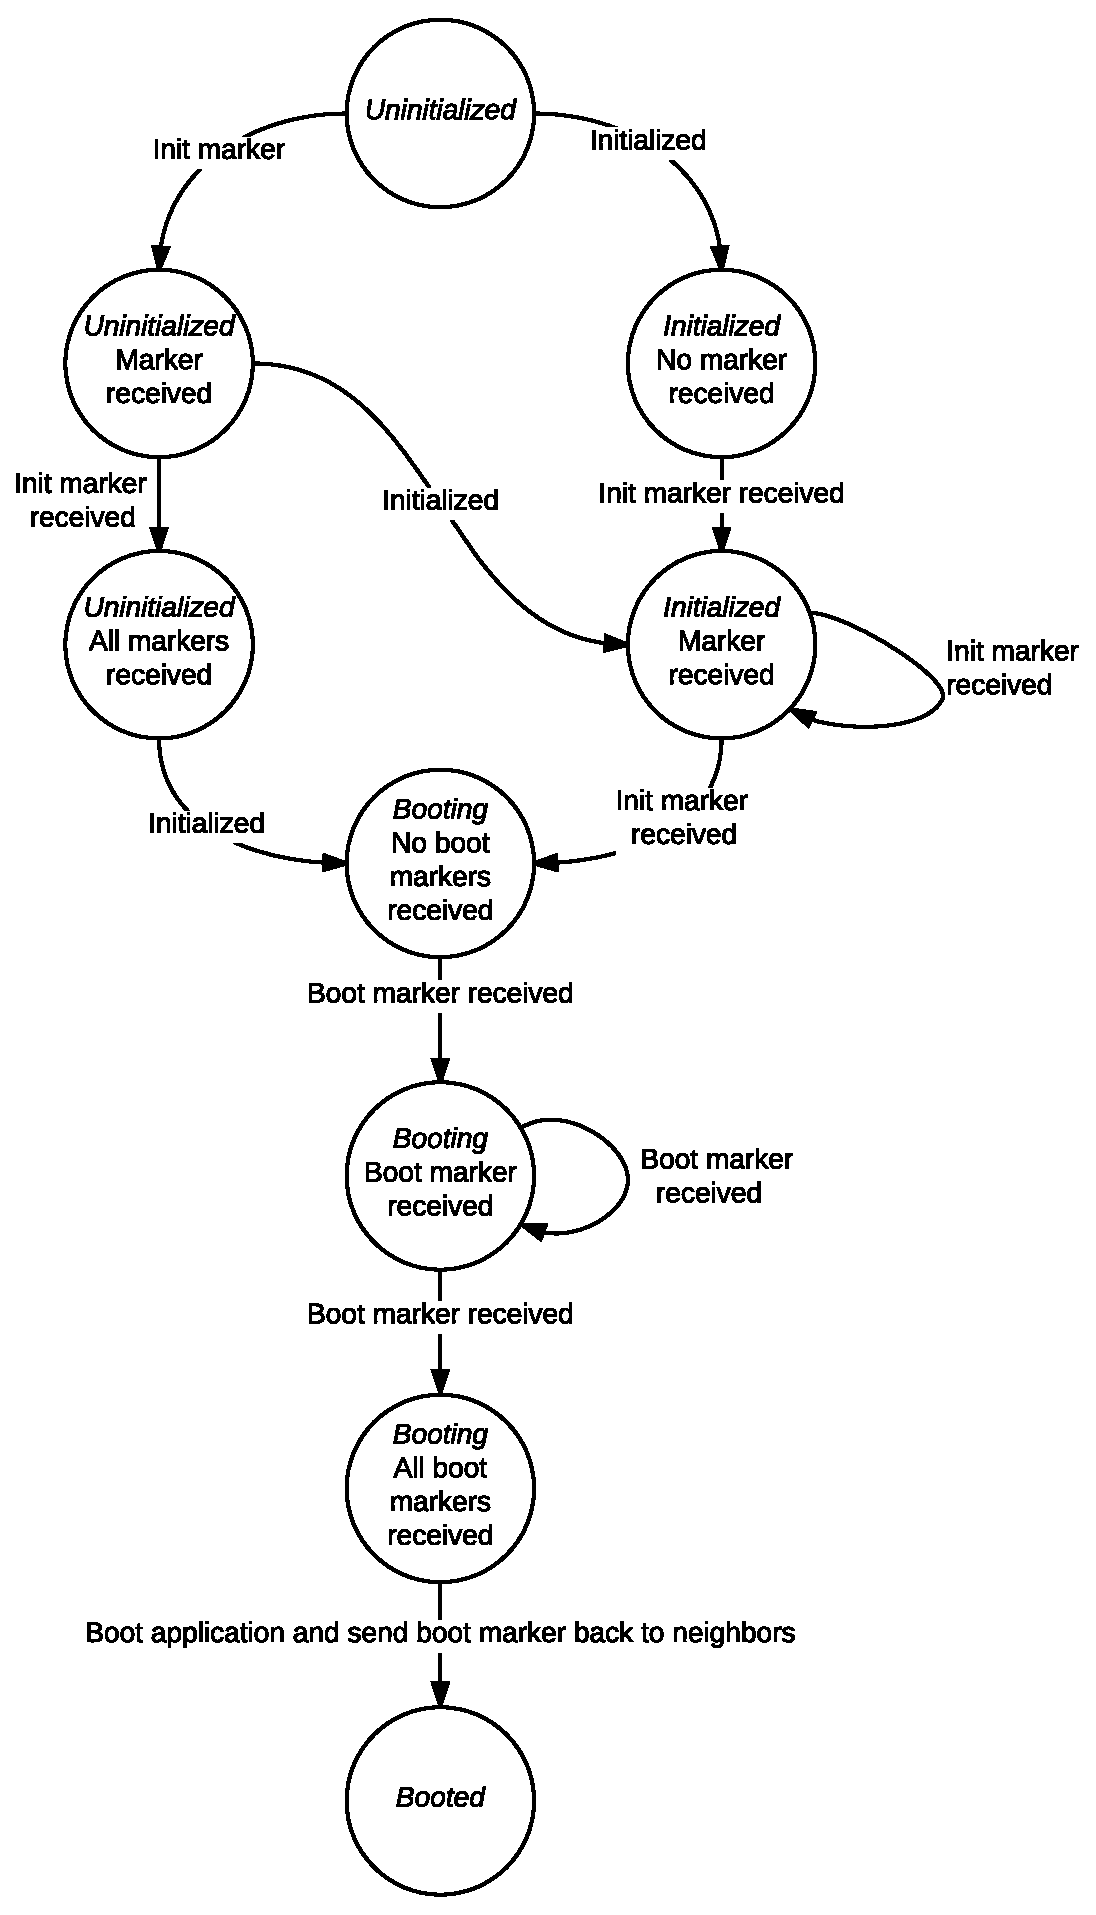
\includegraphics[width=.8\columnwidth]{images/solution/mw/boot.eps}
  \caption{Boot service: activity diagram}
  \label{fig:mw-boot}
\end{figure}
